\begin{enumerate}[label=\thesection.\arabic*,ref=\thesection.\theenumi]
\numberwithin{equation}{enumi}
\numberwithin{figure}{enumi}
\numberwithin{table}{enumi}
\item  $\vec{A},\vec{B},\vec{C}$ are the three points with centre $\vec{O}$ such that $\angle$BOC=30\degree and $\angle$AOB=60\degree. If $\vec{D}$ is a point on the circle other than the arc ABC, find $\angle$ADC.
\label{chapters/9/10/5/1}
\\
\solution
\iffalse
\documentclass[12pt]{article}
\usepackage{graphicx}
\usepackage{amsmath}
\usepackage{mathtools}
\usepackage{gensymb}

\newcommand{\mydet}[1]{\ensuremath{\begin{vmatrix}#1\end{vmatrix}}}
\providecommand{\brak}[1]{\ensuremath{\left(#1\right)}}
\providecommand{\norm}[1]{\left\lVert#1\right\rVert}
\newcommand{\solution}{\noindent \textbf{Solution: }}
\newcommand{\myvec}[1]{\ensuremath{\begin{pmatrix}#1\end{pmatrix}}}
\let\vec\mathbf
\def\inputGnumericTable{}
\usepackage{color}                                            %%
    \usepackage{array}                                            %%
    \usepackage{longtable}                                        %%
    \usepackage{calc}                                             %%
    \usepackage{multirow}                                         %%
    \usepackage{hhline}                                           %%
    \usepackage{ifthen}
\usepackage{array}
\usepackage{amsmath}   % for having text in math mode
\usepackage{listings}
\lstset{
language=tex,
frame=single, 
breaklines=true
}
\begin{document}
\begin{center}
\textbf\large{CLASS-9\\CHAPTER-10 \\ CIRCLES}

\end{center}
\section*{Excercise 10.5}

Q1. section*{\large Solution}
\fi
\begin{figure}[h!]
\centering
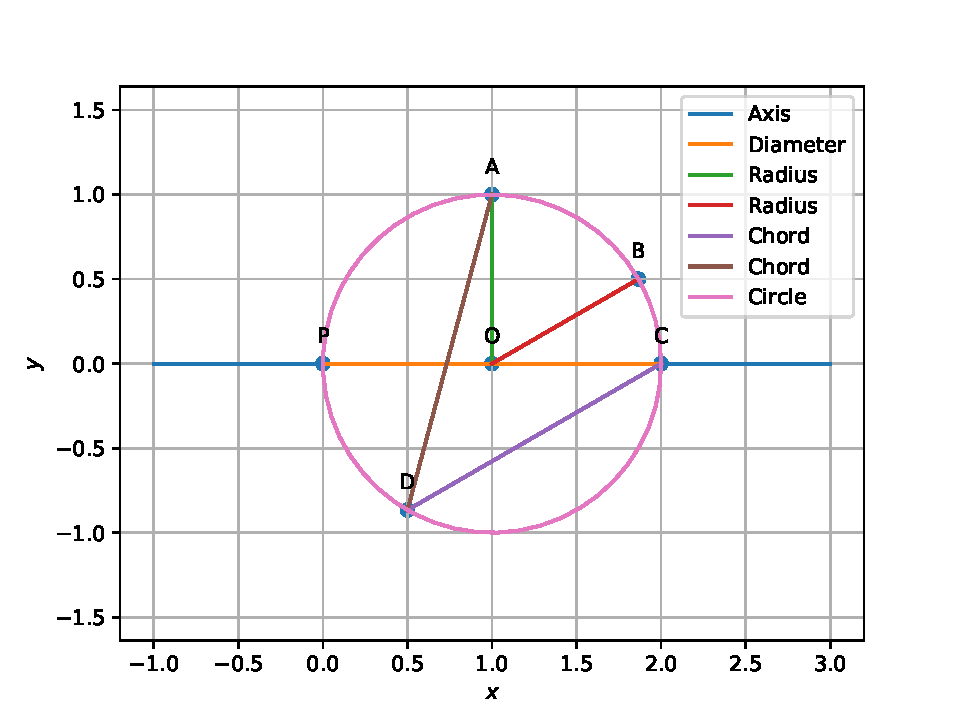
\includegraphics[width=\columnwidth]{chapters/9/10/5/1/figs/circle1.pdf}
\caption{}
\label{fig:chapters/9/10/5/1/Fig1}
\end{figure}
%
\begin{table}[h!]
	\centering
	%\subimport{../chapters/9/10/5/1/tables/}{table1.tex}
     %%%%%%%%%%%%%%%%%%%%%%%%%%%%%%%%%%%%%%%%%%%%%%%%%%%%%%%%%%%%%%%%%%%%%%
%%                                                                  %%
%%  This is the header of a LaTeX2e file exported from Gnumeric.    %%
%%                                                                  %%
%%  This file can be compiled as it stands or included in another   %%
%%  LaTeX document. The table is based on the longtable package so  %%
%%  the longtable options (headers, footers...) can be set in the   %%
%%  preamble section below (see PRAMBLE).                           %%
%%                                                                  %%
%%  To include the file in another, the following two lines must be %%
%%  in the including file:                                          %%
%%        \def\inputGnumericTable{}                                 %%
%%  at the beginning of the file and:                               %%
%%        \input{name-of-this-file.tex}                             %%
%%  where the table is to be placed. Note also that the including   %%
%%  file must use the following packages for the table to be        %%
%%  rendered correctly:                                             %%
%%    \usepackage[latin1]{inputenc}                                 %%
%%    \usepackage{color}                                            %%
%%    \usepackage{array}                                            %%
%%    \usepackage{longtable}                                        %%
%%    \usepackage{calc}                                             %%
%%    \usepackage{multirow}                                         %%
%%    \usepackage{hhline}                                           %%
%%    \usepackage{ifthen}                                           %%
%%  optionally (for landscape tables embedded in another document): %%
%%    \usepackage{lscape}                                           %%
%%                                                                  %%
%%%%%%%%%%%%%%%%%%%%%%%%%%%%%%%%%%%%%%%%%%%%%%%%%%%%%%%%%%%%%%%%%%%%%



%%  This section checks if we are begin input into another file or  %%
%%  the file will be compiled alone. First use a macro taken from   %%
%%  the TeXbook ex 7.7 (suggestion of Han-Wen Nienhuys).            %%
\def\ifundefined#1{\expandafter\ifx\csname#1\endcsname\relax}


%%  Check for the \def token for inputed files. If it is not        %%
%%  defined, the file will be processed as a standalone and the     %%
%%  preamble will be used.                                          %%
\ifundefined{inputGnumericTable}

%%  We must be able to close or not the document at the end.        %%
	\def\gnumericTableEnd{\end{document}}


%%%%%%%%%%%%%%%%%%%%%%%%%%%%%%%%%%%%%%%%%%%%%%%%%%%%%%%%%%%%%%%%%%%%%%
%%                                                                  %%
%%  This is the PREAMBLE. Change these values to get the right      %%
%%  paper size and other niceties.                                  %%
%%                                                                  %%
%%%%%%%%%%%%%%%%%%%%%%%%%%%%%%%%%%%%%%%%%%%%%%%%%%%%%%%%%%%%%%%%%%%%%%

	\documentclass[12pt%
			  %,landscape%
                    ]{report}
       \usepackage[latin1]{inputenc}
       \usepackage{fullpage}
       \usepackage{color}
       \usepackage{array}
       \usepackage{longtable}
       \usepackage{calc}
       \usepackage{multirow}
       \usepackage{hhline}
       \usepackage{ifthen}
       \usepackage{gensymb}
       \usepackage{graphicx}
\usepackage{amsmath}
\usepackage{mathtools}
\newcommand{\mydet}[1]{\ensuremath{\begin{vmatrix}#1\end{vmatrix}}}
\providecommand{\brak}[1]{\ensuremath{\left(#1\right)}}
\providecommand{\norm}[1]{\left\lVert#1\right\rVert}
\newcommand{\solution}{\noindent \textbf{Solution: }}
\newcommand{\myvec}[1]{\ensuremath{\begin{pmatrix}#1\end{pmatrix}}}
\let\vec\mathbf
	\begin{document}


%%  End of the preamble for the standalone. The next section is for %%
%%  documents which are included into other LaTeX2e files.          %%
\else

%%  We are not a stand alone document. For a regular table, we will %%
%%  have no preamble and only define the closing to mean nothing.   %%
    \def\gnumericTableEnd{}

%%  If we want landscape mode in an embedded document, comment out  %%
%%  the line above and uncomment the two below. The table will      %%
%%  begin on a new page and run in landscape mode.                  %%
%       \def\gnumericTableEnd{\end{landscape}}
%       \begin{landscape}


%%  End of the else clause for this file being \input.              %%
\fi

%%%%%%%%%%%%%%%%%%%%%%%%%%%%%%%%%%%%%%%%%%%%%%%%%%%%%%%%%%%%%%%%%%%%%%
%%                                                                  %%
%%  The rest is the gnumeric table, except for the closing          %%
%%  statement. Changes below will alter the table's appearance.     %%
%%                                                                  %%
%%%%%%%%%%%%%%%%%%%%%%%%%%%%%%%%%%%%%%%%%%%%%%%%%%%%%%%%%%%%%%%%%%%%%%
\providecommand{\gnumericmathit}[1]{#1} 
%%  Uncomment the next line if you would like your numbers to be in %%
%%  italics if they are italizised in the gnumeric table.           %%
%\renewcommand{\gnumericmathit}[1]{\mathit{#1}}
\providecommand{\gnumericPB}[1]%
{\let\gnumericTemp=\\#1\let\\=\gnumericTemp\hspace{0pt}}
 \ifundefined{gnumericTableWidthDefined}
        \newlength{\gnumericTableWidth}
        \newlength{\gnumericTableWidthComplete}
        \newlength{\gnumericMultiRowLength}
        \global\def\gnumericTableWidthDefined{}
 \fi
%% The following setting protects this code from babel shorthands.  %%
 \ifthenelse{\isundefined{\languageshorthands}}{}{\languageshorthands{english}}
%%  The default table format retains the relative column widths of  %%
%%  gnumeric. They can easily be changed to c, r or l. In that case %%
%%  you may want to comment out the next line and uncomment the one %%
%%  thereafter                                                      %%
\providecommand\gnumbox{\makebox[0pt]}
%%\providecommand\gnumbox[1][]{\makebox}

%% to adjust positions in multirow situations                       %%
\setlength{\bigstrutjot}{\jot}
\setlength{\extrarowheight}{\doublerulesep}

%%  The \setlongtables command keeps column widths the same across  %%
%%  pages. Simply comment out next line for varying column widths.  %%
\setlongtables

\setlength\gnumericTableWidth{%
	40pt+%
	35pt+%
	210pt+%
0pt}
\def\gumericNumCols{3}
\setlength\gnumericTableWidthComplete{\gnumericTableWidth+%
         \tabcolsep*\gumericNumCols*2+\arrayrulewidth*\gumericNumCols}
\ifthenelse{\lengthtest{\gnumericTableWidthComplete > \linewidth}}%
         {\def\gnumericScale{\ratio{\linewidth-%
                        \tabcolsep*\gumericNumCols*2-%
                        \arrayrulewidth*\gumericNumCols}%
{\gnumericTableWidth}}}%
{\def\gnumericScale{1}}

%%%%%%%%%%%%%%%%%%%%%%%%%%%%%%%%%%%%%%%%%%%%%%%%%%%%%%%%%%%%%%%%%%%%%%
%%                                                                  %%
%% The following are the widths of the various columns. We are      %%
%% defining them here because then they are easier to change.       %%
%% Depending on the cell formats we may use them more than once.    %%
%%                                                                  %%
%%%%%%%%%%%%%%%%%%%%%%%%%%%%%%%%%%%%%%%%%%%%%%%%%%%%%%%%%%%%%%%%%%%%%%

\ifthenelse{\isundefined{\gnumericColA}}{\newlength{\gnumericColA}}{}\settowidth{\gnumericColA}{\begin{tabular}{@{}p{40pt*\gnumericScale}@{}}x\end{tabular}}
\ifthenelse{\isundefined{\gnumericColB}}{\newlength{\gnumericColB}}{}\settowidth{\gnumericColB}{\begin{tabular}{@{}p{35pt*\gnumericScale}@{}}x\end{tabular}}
\ifthenelse{\isundefined{\gnumericColC}}{\newlength{\gnumericColC}}{}\settowidth{\gnumericColC}{\begin{tabular}{@{}p{210pt*\gnumericScale}@{}}x\end{tabular}}

\begin{longtable}[c]{%
	b{\gnumericColA}%
	b{\gnumericColB}%
	b{\gnumericColC}%
	}

%%%%%%%%%%%%%%%%%%%%%%%%%%%%%%%%%%%%%%%%%%%%%%%%%%%%%%%%%%%%%%%%%%%%%%
%%  The longtable options. (Caption, headers... see Goosens, p.124) %%
%	\caption{The Table Caption.}             \\	%
% \hline	% Across the top of the table.
%%  The rest of these options are table rows which are placed on    %%
%%  the first, last or every page. Use \multicolumn if you want.    %%

%%  Header for the first page.                                      %%
%	\multicolumn{3}{c}{The First Header} \\ \hline 
%	\multicolumn{1}{c}{colTag}	%Column 1
%	&\multicolumn{1}{c}{colTag}	%Column 2
%	&\multicolumn{1}{c}{colTag}	\\ \hline %Last column
%	\endfirsthead

%%  The running header definition.                                  %%
%	\hline
%	\multicolumn{3}{l}{\ldots\small\slshape continued} \\ \hline
%	\multicolumn{1}{c}{colTag}	%Column 1
%	&\multicolumn{1}{c}{colTag}	%Column 2
%	&\multicolumn{1}{c}{colTag}	\\ \hline %Last column
%	\endhead

%%  The running footer definition.                                  %%
%	\hline
%	\multicolumn{3}{r}{\small\slshape continued\ldots} \\
%	\endfoot

%%  The ending footer definition.                                   %%
%	\multicolumn{3}{c}{That's all folks} \\ \hline 
%	\endlastfoot
%%%%%%%%%%%%%%%%%%%%%%%%%%%%%%%%%%%%%%%%%%%%%%%%%%%%%%%%%%%%%%%%%%%%%%

\hhline{|-|-|-}
	 \multicolumn{1}{|p{\gnumericColA}|}%
	{\gnumericPB{\raggedright}\gnumbox[l]{\textbf{Symbol}}}
	&\multicolumn{1}{p{\gnumericColB}|}%
	{\gnumericPB{\raggedright}\gnumbox[l]{\textbf{Values}}}
	&\multicolumn{1}{p{\gnumericColC}|}%
	{\gnumericPB{\raggedright}\gnumbox[l]{\textbf{Description}}}
\\
\hhline{|---|}
	 \multicolumn{1}{|p{\gnumericColA}|}%
	{\gnumericPB{\raggedright}\gnumbox[l]{r}}
	&\multicolumn{1}{p{\gnumericColB}|}%
	{\gnumericPB{\raggedright}\gnumbox[l]{1 unit}}
	&\multicolumn{1}{p{\gnumericColC}|}%
	{\gnumericPB{\raggedright}\gnumbox[l]{Radius of OA and OB}}
\\
\hhline{|---|}
	 \multicolumn{1}{|p{\gnumericColA}|}%
	{\gnumericPB{\raggedright}\gnumbox[l]{$\vec{O}$}}
	&\multicolumn{1}{p{\gnumericColB}|}%
	{\gnumericPB{\raggedright}\gnumbox[l]{\myvec{0\\0}}}
	&\multicolumn{1}{p{\gnumericColC}|}%
	{\gnumericPB{\raggedright}\gnumbox[l]{Center of the circle }}
\\
\hhline{|---|}
	 \multicolumn{1}{|p{\gnumericColA}|}%
	{\gnumericPB{\raggedright}\gnumbox[l]{$\vec{C}$}}
	&\multicolumn{1}{p{\gnumericColB}|}%
	{\gnumericPB{\raggedright}\gnumbox[l]{\myvec{1\\0}}}
	&\multicolumn{1}{p{\gnumericColC}|}%
	{\gnumericPB{\raggedright}\gnumbox[l]{Standard basis vector $\vec{e}_1$}}
\\
\hhline{|---|}
	 \multicolumn{1}{|p{\gnumericColA}|}%
	{\gnumericPB{\raggedright}\gnumbox[l]{$\alpha$}}
	&\multicolumn{1}{p{\gnumericColB}|}%
	{\gnumericPB{\raggedright}\gnumbox[l]{30\degree}}
	&\multicolumn{1}{p{\gnumericColC}|}%
	{\gnumericPB{\raggedright}\gnumbox[l]{$\angle$BOC}}
\\
\hhline{|---|}
	 \multicolumn{1}{|p{\gnumericColA}|}%
	{\gnumericPB{\raggedright}\gnumbox[l]{$\beta$}}
	&\multicolumn{1}{p{\gnumericColB}|}%
	{\gnumericPB{\raggedright}\gnumbox[l]{60\degree}}
	&\multicolumn{1}{p{\gnumericColC}|}%
	{\gnumericPB{\raggedright}\gnumbox[l]{$\angle$AOB}}
\\
\hhline{|---|}
	 \multicolumn{1}{|p{\gnumericColA}|}%
	{\gnumericPB{\raggedright}\gnumbox[l]{\textbf{$\gamma$}}}
	&\multicolumn{1}{p{\gnumericColB}|}%
	{\gnumericPB{\raggedright}\gnumbox[l]{??}}
	&\multicolumn{1}{p{\gnumericColC}|}%
	{\gnumericPB{\raggedright}\gnumbox[l]{$\angle$ADC}}
\\
\hhline{|-|-|-|}
\end{longtable}

\ifthenelse{\isundefined{\languageshorthands}}{}{\languageshorthands{\languagename}}
\gnumericTableEnd%

%	\caption{}
	\label{table:chapters/9/10/5/1/table1}
	\end{table}
The input parameters are available in Table
	\ref{table:chapters/9/10/5/1/table1} yielding
\begin{align}
	\vec{C} =\vec{e}_1= \myvec{1\\0},\,
	\vec{A} = \myvec{\cos(\alpha+\beta)\\\sin(\alpha+\beta)},\,
	\vec{D} = \myvec{\cos\gamma\\\sin\gamma}.
\end{align}
Since
\begin{align}
	 \vec{A-D}& = \myvec{\cos(\alpha+\beta) - \cos\gamma\\\sin(\alpha+\beta) - \sin\gamma},
	 \vec{C-D} &= \myvec{1 - \cos\gamma\\-\sin\gamma},
	 \norm{\vec{A-D}}\norm{\vec{C-D}}& = 4 \sin\frac{\alpha+\gamma}2\sin\frac{\beta+\gamma}2,
	 \\
	\cos(\angle ADC) &= \frac{\vec{(A-D)^\top(C-D)}}{\norm{\vec{A-D}}\norm{\vec{C-D}}},
	\label{eq:2}
	\\
	&= 4\sin\frac{\alpha+\gamma}2\sin\frac{\beta+\gamma}2\cos\frac{\alpha+\beta}2
 = \cos\frac{\alpha+\beta}{2}
	\label{eq:7}
\end{align}
Substituting $\alpha$ and $\beta$ in \eqref{eq:7}
\begin{align}
\angle ADC = \frac{\alpha+\beta}{2}=\frac{(30\degree + 60\degree )}{2}=45\degree
\end{align}
See Fig. 
\ref{fig:chapters/9/10/5/1/Fig1}.



\item A chord of a circle is equal to the radius of the circle. Find the angle subtended by the chord at a point on the minor arc and also at a point on the major arc.
\label{chapters/9/10/5/2}
\\
\solution
\documentclass[12pt]{article}
\usepackage{graphicx}
\usepackage{amsmath}
\usepackage{mathtools}
\usepackage{gensymb}
\usepackage[latin1]{inputenc}
\usepackage{fullpage}
\usepackage{color}
\usepackage{array}
\usepackage{longtable}
\usepackage{calc}
\usepackage{multirow}
\usepackage{hhline}
\usepackage{ifthen}
\usepackage{booktabs}
\usepackage{graphicx}
\def\inputGnumericTable{}

\newcommand{\mydet}[1]{\ensuremath{\begin{vmatrix}#1\end{vmatrix}}}
\providecommand{\brak}[1]{\ensuremath{\left(#1\right)}}
\providecommand{\norm}[1]{\left\lVert#1\right\rVert}
\newcommand{\solution}{\noindent \textbf{Solution: }}
\newcommand{\myvec}[1]{\ensuremath{\begin{pmatrix}#1\end{pmatrix}}}
\let\vec\mathbf

\begin{document}
\begin{center}
\textbf\large{CHAPTER-9 \\ CIRCLES}

\end{center}
\begin{enumerate}
\section{EXERCISE-10.5}
\item A chord of a circle is equal to the radius of the circle. Find the angle subtended by the chord at a point on the minor arc and also at a point on the major arc.
\section{SOLUTION}
The input parameters are\\
\begin{table}[h!]
	%%%%%%%%%%%%%%%%%%%%%%%%%%%%%%%%%%%%%%%%%%%%%%%%%%%%%%%%%%%%%%%%%%%%%%
%%                                                                  %%
%%  This is the header of a LaTeX2e file exported from Gnumeric.    %%
%%                                                                  %%
%%  This file can be compiled as it stands or included in another   %%
%%  LaTeX document. The table is based on the longtable package so  %%
%%  the longtable options (headers, footers...) can be set in the   %%
%%  preamble section below (see PRAMBLE).                           %%
%%                                                                  %%
%%  To include the file in another, the following two lines must be %%
%%  in the including file:                                          %%
%%        \def\inputGnumericTable{}                                 %%
%%  at the beginning of the file and:                               %%
%%        \input{name-of-this-file.tex}                             %%
%%  where the table is to be placed. Note also that the including   %%
%%  file must use the following packages for the table to be        %%
%%  rendered correctly:                                             %%
%%    \usepackage[latin1]{inputenc}                                 %%
%%    \usepackage{color}                                            %%
%%    \usepackage{array}                                            %%
%%    \usepackage{longtable}                                        %%
%%    \usepackage{calc}                                             %%
%%    \usepackage{multirow}                                         %%
%%    \usepackage{hhline}                                           %%
%%    \usepackage{ifthen}                                           %%
%%  optionally (for landscape tables embedded in another document): %%
%%    \usepackage{lscape}                                           %%
%%                                                                  %%
%%%%%%%%%%%%%%%%%%%%%%%%%%%%%%%%%%%%%%%%%%%%%%%%%%%%%%%%%%%%%%%%%%%%%%



%%  This section checks if we are begin input into another file or  %%
%%  the file will be compiled alone. First use a macro taken from   %%
%%  the TeXbook ex 7.7 (suggestion of Han-Wen Nienhuys).            %%
\def\ifundefined#1{\expandafter\ifx\csname#1\endcsname\relax}


%%  Check for the \def token for inputed files. If it is not        %%
%%  defined, the file will be processed as a standalone and the     %%
%%  preamble will be used.                                          %%
\ifundefined{inputGnumericTable}

%%  We must be able to close or not the document at the end.        %%
	\def\gnumericTableEnd{\end{document}}


%%%%%%%%%%%%%%%%%%%%%%%%%%%%%%%%%%%%%%%%%%%%%%%%%%%%%%%%%%%%%%%%%%%%%%
%%                                                                  %%
%%  This is the PREAMBLE. Change these values to get the right      %%
%%  paper size and other niceties.                                  %%
%%                                                                  %%
%%%%%%%%%%%%%%%%%%%%%%%%%%%%%%%%%%%%%%%%%%%%%%%%%%%%%%%%%%%%%%%%%%%%%%

	\documentclass[12pt%
			  %,landscape%
                    ]{report}
       \usepackage[latin1]{inputenc}
       \usepackage{fullpage}
       \usepackage{color}
       \usepackage{array}
       \usepackage{longtable}
       \usepackage{calc}
       \usepackage{multirow}
       \usepackage{hhline}
       \usepackage{ifthen}

	\begin{document}


%%  End of the preamble for the standalone. The next section is for %%
%%  documents which are included into other LaTeX2e files.          %%
\else

%%  We are not a stand alone document. For a regular table, we will %%
%%  have no preamble and only define the closing to mean nothing.   %%
    \def\gnumericTableEnd{}

%%  If we want landscape mode in an embedded document, comment out  %%
%%  the line above and uncomment the two below. The table will      %%
%%  begin on a new page and run in landscape mode.                  %%
%       \def\gnumericTableEnd{\end{landscape}}
%       \begin{landscape}


%%  End of the else clause for this file being \input.              %%
\fi

%%%%%%%%%%%%%%%%%%%%%%%%%%%%%%%%%%%%%%%%%%%%%%%%%%%%%%%%%%%%%%%%%%%%%%
%%                                                                  %%
%%  The rest is the gnumeric table, except for the closing          %%
%%  statement. Changes below will alter the table's appearance.     %%
%%                                                                  %%
%%%%%%%%%%%%%%%%%%%%%%%%%%%%%%%%%%%%%%%%%%%%%%%%%%%%%%%%%%%%%%%%%%%%%%

\providecommand{\gnumericmathit}[1]{#1} 
%%  Uncomment the next line if you would like your numbers to be in %%
%%  italics if they are italizised in the gnumeric table.           %%
%\renewcommand{\gnumericmathit}[1]{\mathit{#1}}
\providecommand{\gnumericPB}[1]%
{\let\gnumericTemp=\\#1\let\\=\gnumericTemp\hspace{0pt}}
 \ifundefined{gnumericTableWidthDefined}
        \newlength{\gnumericTableWidth}
        \newlength{\gnumericTableWidthComplete}
        \newlength{\gnumericMultiRowLength}
        \global\def\gnumericTableWidthDefined{}
 \fi
%% The following setting protects this code from babel shorthands.  %%
 \ifthenelse{\isundefined{\languageshorthands}}{}{\languageshorthands{english}}
%%  The default table format retains the relative column widths of  %%
%%  gnumeric. They can easily be changed to c, r or l. In that case %%
%%  you may want to comment out the next line and uncomment the one %%
%%  thereafter                                                      %%
\providecommand\gnumbox{\makebox[0pt]}
%%\providecommand\gnumbox[1][]{\makebox}

%% to adjust positions in multirow situations                       %%
\setlength{\bigstrutjot}{\jot}
\setlength{\extrarowheight}{\doublerulesep}

%%  The \setlongtables command keeps column widths the same across  %%
%%  pages. Simply comment out next line for varying column widths.  %%
\setlongtables

\setlength\gnumericTableWidth{%
	53pt+%
	53pt+%
	82pt+%
	53pt+%
0pt}
\def\gumericNumCols{4}
\setlength\gnumericTableWidthComplete{\gnumericTableWidth+%
         \tabcolsep*\gumericNumCols*2+\arrayrulewidth*\gumericNumCols}
\ifthenelse{\lengthtest{\gnumericTableWidthComplete > \linewidth}}%
         {\def\gnumericScale{1*\ratio{\linewidth-%
                        \tabcolsep*\gumericNumCols*2-%
                        \arrayrulewidth*\gumericNumCols}%
{\gnumericTableWidth}}}%
{\def\gnumericScale{1}}

%%%%%%%%%%%%%%%%%%%%%%%%%%%%%%%%%%%%%%%%%%%%%%%%%%%%%%%%%%%%%%%%%%%%%%
%%                                                                  %%
%% The following are the widths of the various columns. We are      %%
%% defining them here because then they are easier to change.       %%
%% Depending on the cell formats we may use them more than once.    %%
%%                                                                  %%
%%%%%%%%%%%%%%%%%%%%%%%%%%%%%%%%%%%%%%%%%%%%%%%%%%%%%%%%%%%%%%%%%%%%%%

\ifthenelse{\isundefined{\gnumericColA}}{\newlength{\gnumericColA}}{}\settowidth{\gnumericColA}{\begin{tabular}{@{}p{53pt*\gnumericScale}@{}}x\end{tabular}}
\ifthenelse{\isundefined{\gnumericColB}}{\newlength{\gnumericColB}}{}\settowidth{\gnumericColB}{\begin{tabular}{@{}p{53pt*\gnumericScale}@{}}x\end{tabular}}
\ifthenelse{\isundefined{\gnumericColC}}{\newlength{\gnumericColC}}{}\settowidth{\gnumericColC}{\begin{tabular}{@{}p{82pt*\gnumericScale}@{}}x\end{tabular}}
\ifthenelse{\isundefined{\gnumericColD}}{\newlength{\gnumericColD}}{}\settowidth{\gnumericColD}{\begin{tabular}{@{}p{53pt*\gnumericScale}@{}}x\end{tabular}}

	\begin{center}
\begin{tabular}[c]{%
	b{\gnumericColA}%
	b{\gnumericColB}%
	b{\gnumericColC}%
	b{\gnumericColD}%
	}

%%%%%%%%%%%%%%%%%%%%%%%%%%%%%%%%%%%%%%%%%%%%%%%%%%%%%%%%%%%%%%%%%%%%%%
%%  The longtable options. (Caption, headers... see Goosens, p.124) %%
%	\caption{The Table Caption.}             \\	%
% \hline	% Across the top of the table.
%%  The rest of these options are table rows which are placed on    %%
%%  the first, last or every page. Use \multicolumn if you want.    %%

%%  Header for the first page.                                      %%
%	\multicolumn{4}{c}{The First Header} \\ \hline 
%	\multicolumn{1}{c}{colTag}	%Column 1
%	&\multicolumn{1}{c}{colTag}	%Column 2
%	&\multicolumn{1}{c}{colTag}	%Column 3
%	&\multicolumn{1}{c}{colTag}	\\ \hline %Last column
%	\endfirsthead

%%  The running header definition.                                  %%
%	\hline
%	\multicolumn{4}{l}{\ldots\small\slshape continued} \\ \hline
%	\multicolumn{1}{c}{colTag}	%Column 1
%	&\multicolumn{1}{c}{colTag}	%Column 2
%	&\multicolumn{1}{c}{colTag}	%Column 3
%	&\multicolumn{1}{c}{colTag}	\\ \hline %Last column
%	\endhead

%%  The running footer definition.                                  %%
%	\hline
%	\multicolumn{4}{r}{\small\slshape continued\ldots} \\
%	\endfoot

%%  The ending footer definition.                                   %%
%	\multicolumn{4}{c}{That's all folks} \\ \hline 
%	\endlastfoot
%%%%%%%%%%%%%%%%%%%%%%%%%%%%%%%%%%%%%%%%%%%%%%%%%%%%%%%%%%%%%%%%%%%%%%

\hhline{|-|-|-~}
	 \multicolumn{1}{|p{\gnumericColA}|}%
	{\gnumericPB{\centering}\gnumbox{\textbf{Symbol}}}
	&\multicolumn{1}{p{\gnumericColB}|}%
	{\gnumericPB{\centering}\gnumbox{\textbf{Value}}}
	&\multicolumn{1}{p{\gnumericColC}|}%
	{\gnumericPB{\centering}\gnumbox{\textbf{Description}}}
	&
\\
\hhline{|---|~}
	 \multicolumn{1}{|p{\gnumericColA}|}%
	{\gnumericPB{\centering}\gnumbox{$\vec{P}$}}
	&\multicolumn{1}{p{\gnumericColB}|}%
	{\gnumericPB{\centering}\gnumbox{$\myvec{5\\-3}$}}
	&\multicolumn{1}{p{\gnumericColC}|}%
	{\gnumericPB{\centering}\gnumbox{First point}}
	&
\\
\hhline{|---|~}
	 \multicolumn{1}{|p{\gnumericColA}|}%
	{\gnumericPB{\centering}\gnumbox{$\vec{Q}$}}
	&\multicolumn{1}{p{\gnumericColB}|}%
	{\gnumericPB{\centering}\gnumbox{$\myvec{0\\1}$}}
	&\multicolumn{1}{p{\gnumericColC}|}%
	{\gnumericPB{\centering}\gnumbox{Second point}}
	&
\\
\hhline{|---|~}
	 \multicolumn{1}{|p{\gnumericColA}|}%
	{\gnumericPB{\centering}\gnumbox{$\vec{R}$}}
	&\multicolumn{1}{p{\gnumericColB}|}%
	{\gnumericPB{\centering}\gnumbox{$\myvec{?\\6}$}}
	&\multicolumn{1}{p{\gnumericColC}|}%
	{\gnumericPB{\centering}\gnumbox{Desired point}}
	&
\\
\hhline{|-|-|-|~}
\end{tabular}
	\end{center}

\ifthenelse{\isundefined{\languageshorthands}}{}{\languageshorthands{\languagename}}
\gnumericTableEnd
\caption{}
\label{table}	
\end{table}
\\
Take three points Q,R and P on a unit circle  at angles $\theta,\alpha,\text{ and }\beta$.Then
\begin{align}
	\vec{Q} = \myvec{\cos\theta\\ \sin\theta},
	\vec{R} = \myvec{\cos\alpha\\ \sin\alpha},
	\vec{S} = \myvec{\cos\beta\\ \sin\beta}
\end{align}
\begin{align}
	\cos\angle QRP&= \frac{\brak{\vec{Q}-\vec{R}}\brak{\vec{P}-\vec{R}}}{\norm{\vec{Q}-\vec{R}}\norm{\vec{P}-\vec{R}}}\label{eq:2}
\end{align}
Where
\begin{align}
\brak{\vec{Q}-\vec{R}}\brak{\vec{P}-\vec{R}}&= \brak{\cos\theta-\cos\alpha}\brak{ \sin\theta-\sin\alpha}\brak{1-\cos\alpha}\brak{0-\sin\alpha}\\
&=\brak{\cos\theta-\cos\alpha}\cos\alpha+\brak{\sin\theta-\sin\alpha}\\
&=2\sin\frac{\theta-\alpha}{2}\sin\frac{\theta+\alpha}{2}\cos\alpha+2\cos\frac{\theta+\alpha}{2}\sin\frac{\theta-\alpha}{2}\\
&=\brak{\cos\alpha-\cos\theta}\cos\alpha+\brak{\sin\theta-\sin\alpha}\label{eq:6}
\end{align}
\begin{align}
\norm{\vec{Q}-\vec{R}}^2\norm{\vec{P}-\vec{R}}^2 &= \brak{\cos\theta-\cos\alpha}^2+\brak{\sin\theta-\sin\alpha}^2
	\brak{1-\cos\alpha}^2+\brak{0-\sin\alpha}^2\\
	&=\brak{2-2\cos\theta\cos\alpha-2\sin\theta\sin\alpha}\brak{2-\cos\alpha}\label{eq:8}
\end{align}
substituing the \eqref{eq:6} and \eqref{eq:8} in \eqref{eq:2}
\begin{align}
\cos\angle QRP&=\frac{2.079}{4.323}\\
\angle QRP&=\cos^{-1}0.480\\
\angle QRP&=62\degree
\end{align}
\begin{align}
\cos\angle QSP&= \frac{\brak{\vec{Q}-\vec{S}}\brak{\vec{P}-\vec{S}}}{\norm{\vec{Q}-\vec{S}}\norm{\vec{P}-\vec{S}}}\label{eq:12}
\end{align}
\begin{align}
\brak{\vec{Q}-\vec{S}}\brak{\vec{P}-\vec{S}}&= \brak{\cos\theta-\cos\beta}\brak{\sin\theta-\sin\beta}\brak{1-\cos\beta}\brak{0-\sin\beta}\\
&=\brak{\cos\theta-\cos\beta}\cos\beta+\brak{\sin\theta-\sin\beta}\\
&=2\sin\frac{\theta-\beta}{2}\sin\frac{\theta+\beta}{2}\cos\beta+2\cos\frac{\theta+\beta}{2}\sin\frac{\theta-\beta}{2}\\
&=\brak{\cos\beta-\cos\theta}\cos\beta+\brak{\sin\theta-\sin\beta}\label{eq:16}
\end{align}
\begin{align}
\norm{\vec{Q}-\vec{S}}^2\norm{\vec{P}-\vec{S}}^2 &= \brak{\cos\theta-\cos\beta}^2+\brak{\sin\theta-\sin\beta}^2
	\brak{1-\cos\beta}^2+\brak{0-\sin\beta}^2\\
	&=\brak{2-2\cos\theta\cos\beta-2\sin\theta\sin\beta}\brak{2-\cos\beta}\label{eq:18}
\end{align}
substituing the \eqref{eq:16} and \eqref{eq:18} in \eqref{eq:12}
\begin{align}
\cos\angle QSP&=\frac{1.048}{1.098}\\
\angle QSP&=\cos^{-1}0.954\\
\angle QSP&=17\degree
\end{align}
\section{FIGURE}
\begin{figure}[h]
\centering
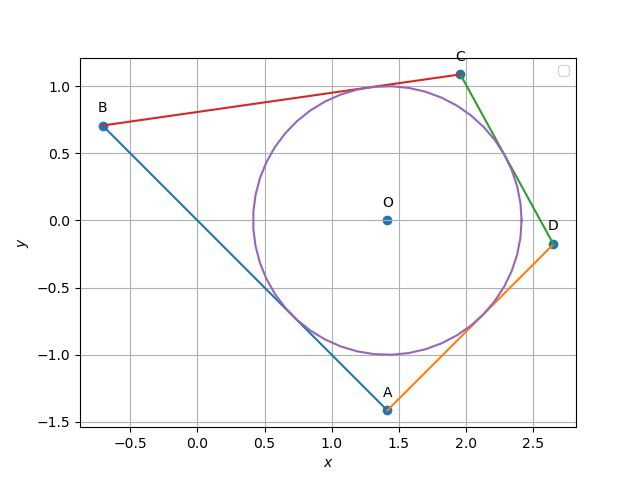
\includegraphics[width=\columnwidth]{circle.png}
\caption{}
		\label{fig:Figure}
\end{figure}
\end{enumerate}
\end{document}

\item 
\label{chapters/9/10/5/3}
\iffalse
\documentclass[journal,10pt,twocolumn]{article}
\usepackage{graphicx, float}
\usepackage[margin=0.5in]{geometry}
\usepackage{amsmath, bm}
\usepackage{array}
\usepackage{booktabs}


\providecommand{\norm}[1]{\left\lVert#1\right\rVert}
\let\vec\mathbf
\newcommand{\myvec}[1]{\ensuremath{\begin{pmatrix}#1\end{pmatrix}}}
\newcommand{\mydet}[1]{\ensuremath{\begin{vmatrix}#1\end{vmatrix}}}

\title{\textbf{Circle Assignment}}
\author{Maddu Dinesh}
\date{September 2022}

\begin{document}

\maketitle
\paragraph{\textit{Problem Statement} -
\fi
Let $\angle PQR = 100\degree$ where $\vec{P}\vec{Q}, \vec{R}$ are points on a circle with centre $\vec{O}$. Find $\angle OPR$.
	\begin{figure}[!ht]
		\centering
 \includegraphics[width=\columnwidth]{chapters/9/10/5/3/figs/fig-1.pdf}
		\caption{}
		\label{fig:9/10/5/3}
  	\end{figure}
	\solution In Fig. 
		\ref{fig:9/10/5/3},
\begin{align}
	\vec{P} = \myvec{\cos\brak{\theta + 160} \\ \sin \brak{\theta + 160}}, \vec{Q} = \myvec{\cos \alpha\\ \sin \alpha}, \vec{R} = \myvec{\cos \theta \\ \sin \theta}.
\end{align}

\iffalse

\section*{\large Solution}

\begin{figure}[H]
\centering
\includegraphics[width=1\columnwidth]{fig-1.pdf}
\label{fig:triangle}
\end{figure}



Given  $\angle$PQR=100°





\section*{ Construction}






{
\setlength\extrarowheight{1pt}


\begin{tabular}{|c|c|c|}
 \hline
 \textbf{Symbol}&\textbf{Value}&\textbf{Description}\\
 \hline
 O&&Centre\\
 \hline
 $\angle$PQR&100$^\circ$&Angle between vectors P and R\\
 \hline
 $\angle$OPR&??&Angle b/w vectors O and R w.r.to P\\
 \hline
 
\end{tabular}

{


\section*{Proof:}
From assumptions the vector points P,Q,R be
\begin{eqnarray}
 \vec{P} = \myvec{cos\theta_1\\sin\theta_1},
 \vec{Q} = \myvec{cos\theta_2\\sin\theta_2},
 \vec{R} = \myvec{cos\theta_3\\sin\theta_3},
 \vec{O} = \myvec{0\\0}
\end{eqnarray}

\begin{align}
 cos(\angle PQR) = \frac{(P-Q)^T(R-Q)}{\norm{P-Q}\norm{R-Q}}
 \label{pf2-eq-1}
\end{align}

Where
 \begin{eqnarray}
 \vec{P-Q} = \myvec{cos\theta_1 - cos\theta_2\\sin\theta_1 - sin\theta_2},
 \vec{R-Q} = \myvec{cos\theta_3 - cos\theta_2\\sin\theta_3 - sin\theta_2}
\end{eqnarray}
 

\begin{eqnarray*}
 (P-Q)^T(R-Q)=\myvec{cos\theta_1 - cos\theta_2  sin\theta_1 - sin\theta_2}
 \myvec{cos\theta_3 - cos\theta_2\\sin\theta_3 - sin\theta_2}
\end{eqnarray*}

\begin{multline*}
 = (\cos\theta_1-\cos\theta_2)(\cos\theta_3-\cos\theta_2)+(\sin\theta_1-\sin\theta_2)(\sin\theta_3-\sin\theta_2)
\end{multline*}

\begin{multline*}
 = -2\sin\frac{\theta_1-\theta_2}2\sin\frac{\theta_1+\theta_2}2 \cdot(-2)\sin\frac{\theta_3-\theta_2}2\sin\frac{\theta_3+\theta_2}2 \\\quad+ 2\cos\frac{\theta_1+\theta_2}2\sin\frac{\theta_1-\theta_2}2 \cdot 2\cos\frac{\theta_2+\theta_3}2\sin\frac{\theta_3-\theta_2}2
\end{multline*}
\begin{multline*}
 = 4\sin\frac{\theta_1-\theta_2}2\sin\frac{\theta_3-\theta_2}2(\sin\frac{\theta_1+\theta_2}2\sin\frac{\theta_3+\theta_2}2+\\
 \cos\frac{\theta_1+\theta_2}2\cos\frac{\theta_3+\theta_2}2)
\end{multline*}
\begin{align*}
 = 4\sin\frac{\theta_1-\theta_2}2\sin\frac{\theta_3-\theta_2}2\cos\left(\frac{\theta_1+\theta_2}2-\frac{\theta_3+\theta_2}2\right)
\end{align*}
\begin{align}
 = 4\sin\frac{\theta_1-\theta_2}2\sin\frac{\theta_3-\theta_2}2\cos\frac{\theta_1-\theta_3}2
 \label{pf2-eq-2}
\end{align}

\begin{multline*}
 \norm{P-Q}^2\norm{R-Q}^2 = ((\cos\theta_1-\cos\theta_2)^2+(\sin\theta_1-\sin\theta_2)^2)\\
 ((\cos\theta_3-\cos\theta_2)^2+(\sin\theta_3-\sin\theta_2)^2)
\end{multline*}
\begin{multline*}
 = (2-2\cos\theta_1\cos\theta_2 - 2\sin\theta_1\sin\theta_2)(2-\\
 2\cos\theta_3\cos\theta_2 - 2\sin\theta_3\sin\theta_2)
\end{multline*}
\begin{align*}
 &= 16 \sin^2\frac{\theta_1-\theta_2}2\sin^2\frac{\theta_3-\theta_2}2
\end{align*}
\begin{align}
 \norm{P-Q}\norm{R-Q} = 4 \sin\frac{\theta_1-\theta_2}2\sin\frac{\theta_3-\theta_2}2
 \label{pf2-eq-3}
\end{align}

Substituting (\ref{pf2-eq-2}) and (\ref{pf2-eq-3}) in (\ref{pf2-eq-1}),
\begin{multline*}
 cos(\angle PQR) = \frac{4sin\frac{\theta_1-\theta_2}{2}sin\frac{\theta_3-\theta_2}{2}cos\frac{\theta_1-\theta_3}{2}}{4 \sin\frac{\theta_1-\theta_2}2\sin\frac{\theta_3-\theta_2}2}
\end{multline*}
\begin{equation}
cos(\angle PQR) = cos\frac{\theta_1-\theta_3}{2}
\label{pf2-eq-4}
\end{equation}
\begin{equation*}
\angle PQR = =\frac{\theta_1 - \theta_3 }{2}=100^\circ
\end{equation*}


\begin{align}
 cos(\angle OPR) = \frac{(P-R)^T(P-O)}{\norm{P-R}\norm{P-O}}
 \label{pf2-eq-5}
\end{align}

\begin{eqnarray}
 \vec{P-R} = \myvec{cos\theta_1 - cos\theta_3\\sin\theta_1 - sin\theta_3},
 \vec{P-O} = \myvec{cos\theta_1 \\sin\theta_1 }
\end{eqnarray}
 

\begin{eqnarray*}
 (P-R)^T(P-O)=\myvec{cos\theta_1 - cos\theta_3\\sin\theta_1 - sin\theta_3}
 \myvec{cos\theta_1 sin\theta_1 }
\end{eqnarray*}

\begin{multline*}
 = (\cos\theta_1-\cos\theta_3)(\cos\theta_1)+(\sin\theta_1-\sin\theta_3)(\sin\theta_1)
\end{multline*}
\begin{multline*}
 = (\cos^2{\theta_1}-\cos\theta_3\cos\theta_1)+(\sin^2{\theta_1}-\sin\theta_1\sin\theta_3)
\end{multline*}
\begin{align*}
 = 1-(\cos\theta_3\cos\theta_1+\sin\theta_1\sin\theta_3)
\end{align*}
\begin{equation}
=1-(cos(\theta_3-\theta_1))
\end{equation}
\begin{multline*}
 \norm{P-R}^2\norm{P-O}^2 = ((\cos\theta_1-\cos\theta_3)^2+(\sin\theta_1-\sin\theta_3)^2)\\
 ((\cos\theta_1)^2+(\sin\theta_1)^2)
\end{multline*}
\begin{align*}
 = 2-2\cos\theta_1\cos\theta_3-2\sin\theta_1\sin\theta_3
\end{align*}
\begin{align*}
 = 2(1-\cos(\theta_1-\theta_3) )
\end{align*}
\begin{align}
 \norm{P-R}\norm{P-O} = \sqrt{2(1-\cos(\theta_1-\theta_3))}
 \label{pf2-eq-6}
\end{align}
\begin{align*}
 cos(\angle OPR) = \frac{(1-\cos(\theta_1-\theta_3)) }{\sqrt{2(1-\cos(\theta_1-\theta_3))}}
\end{align*}
\begin{align*}
\cos(\angle OPR)=0.98
\end{align*}
\begin{align}
\angle OPR=10^\circ
\end{align}






\end{document}
Footer
\fi

    \item Prove that a cyclic paralellogram is a rectangle.
\label{chapters/9/10/5/12}
\\
\solution
\iffalse
\documentclass[journal,12pt,twocolumn]{IEEEtran}
\usepackage{setspace}
\usepackage{gensymb}
\usepackage{xcolor}
\usepackage{caption}
\singlespacing
\usepackage{siunitx}
\usepackage[cmex10]{amsmath}
\usepackage{mathtools}
\usepackage{hyperref}
\usepackage{amsthm}
\usepackage{mathrsfs}
\usepackage{txfonts}
\usepackage{stfloats}
\usepackage{cite}
\usepackage{cases}
\usepackage{subfig}
\usepackage{longtable}
\usepackage{multirow}
\usepackage{enumitem}
\usepackage{bm}
\usepackage{mathtools}
\usepackage{listings}
\usepackage{tikz}
\usetikzlibrary{shapes,arrows,positioning}
\usepackage{circuitikz}
\renewcommand{\vec}[1]{\boldsymbol{\mathbf{#1}}}
\DeclareMathOperator*{\Res}{Res}
\renewcommand\thesection{\arabic{section}}
\renewcommand\thesubsection{\thesection.\arabic{subsection}}
\renewcommand\thesubsubsection{\thesubsection.\arabic{subsubsection}}

\renewcommand\thesectiondis{\arabic{section}}
\renewcommand\thesubsectiondis{\thesectiondis.\arabic{subsection}}
\renewcommand\thesubsubsectiondis{\thesubsectiondis.\arabic{subsubsection}}
\hyphenation{op-tical net-works semi-conduc-tor}

\lstset{
language=Python,
frame=single, 
breaklines=true,
columns=fullflexible
}
\begin{document}
\theoremstyle{definition}
\newtheorem{theorem}{Theorem}[section]
\newtheorem{problem}{Problem}
\newtheorem{proposition}{Proposition}[section]
\newtheorem{lemma}{Lemma}[section]
\newtheorem{corollary}[theorem]{Corollary}
\newtheorem{example}{Example}[section]
\newtheorem{definition}{Definition}[section]
\newcommand{\BEQA}{\begin{eqnarray}}
\newcommand{\EEQA}{\end{eqnarray}}
\newcommand{\define}{\stackrel{\triangle}{=}}
\newcommand{\myvec}[1]{\ensuremath{\begin{pmatrix}#1\end{pmatrix}}}
\newcommand{\mydet}[1]{\ensuremath{\begin{vmatrix}#1\end{vmatrix}}}
\bibliographystyle{IEEEtran}
\providecommand{\nCr}[2]{\,^{#1}C_{#2}} % nCr
\providecommand{\nPr}[2]{\,^{#1}P_{#2}} % nPr
\providecommand{\mbf}{\mathbf}
\providecommand{\pr}[1]{\ensuremath{\Pr\left(#1\right)}}
\providecommand{\qfunc}[1]{\ensuremath{Q\left(#1\right)}}
\providecommand{\sbrak}[1]{\ensuremath{{}\left[#1\right]}}
\providecommand{\lsbrak}[1]{\ensuremath{{}\left[#1\right.}}
\providecommand{\rsbrak}[1]{\ensuremath{{}\left.#1\right]}}
\providecommand{\brak}[1]{\ensuremath{\left(#1\right)}}
\providecommand{\lbrak}[1]{\ensuremath{\left(#1\right.}}
\providecommand{\rbrak}[1]{\ensuremath{\left.#1\right)}}
\providecommand{\cbrak}[1]{\ensuremath{\left\{#1\right\}}}
\providecommand{\lcbrak}[1]{\ensuremath{\left\{#1\right.}}
\providecommand{\rcbrak}[1]{\ensuremath{\left.#1\right\}}}
\theoremstyle{remark}
\newtheorem{rem}{Remark}
\newcommand{\sgn}{\mathop{\mathrm{sgn}}}
\newcommand{\rect}{\mathop{\mathrm{rect}}}
\newcommand{\sinc}{\mathop{\mathrm{sinc}}}
\providecommand{\abs}[1]{\left\vert#1\right\vert}
\providecommand{\res}[1]{\Res\displaylimits_{#1}} 
\providecommand{\norm}[1]{\left\Vert#1\right\Vert}
\providecommand{\mtx}[1]{\mathbf{#1}}
\providecommand{\mean}[1]{E\left[ #1 \right]}
\providecommand{\fourier}{\overset{\mathcal{F}}{ \rightleftharpoons}}
\providecommand{\ztrans}{\overset{\mathcal{Z}}{ \rightleftharpoons}}
\providecommand{\system}[1]{\overset{\mathcal{#1}}{ \longleftrightarrow}}
\newcommand{\solution}{\noindent \textbf{Solution: }}
\providecommand{\dec}[2]{\ensuremath{\overset{#1}{\underset{#2}{\gtrless}}}}
\let\StandardTheFigure\thefigure
\def\putbox#1#2#3{\makebox[0in][l]{\makebox[#1][l]{}\raisebox{\baselineskip}[0in][0in]{\raisebox{#2}[0in][0in]{#3}}}}
     \def\rightbox#1{\makebox[0in][r]{#1}}
     \def\centbox#1{\makebox[0in]{#1}}
     \def\topbox#1{\raisebox{-\baselineskip}[0in][0in]{#1}}
     \def\midbox#1{\raisebox{-0.5\baselineskip}[0in][0in]{#1}}

\vspace{3cm}
\title{Circle Assignment}
\author{Gautam Singh}
\maketitle
\bigskip

\begin{abstract}
    This document contains the solution to Question 12 of 
    Exercise 5 in Chapter 10 of the class 9 NCERT textbook.
\end{abstract}

\begin{enumerate}

    \solution 
\fi
		Consider the points $\vec{P_i},\ 1 \le i \le 4$ in anticlockwise 
    order on the unit circle. Thus, for $1 \le i \le 4$,
    \begin{align}
        \vec{P_i} = \myvec{\cos\theta_i\\\sin\theta_i} 
        \label{eq:chapters/9/10/5/12/circ-point}
    \end{align}
    where 
    \begin{align}
        \theta_i \in [0,2\pi),\ i \neq j \iff \theta_i \neq \theta_j
        \label{eq:chapters/9/10/5/12/theta-cond}
    \end{align}
    Without loss of generality, suppose that $P_1P_2$ and $P_3P_4$ are parallel 
    to the $x$-axis. Since
    \begin{align}
        \vec{P_1}-\vec{P_2} &= \myvec{\cos\theta_1-\cos\theta_2\\\sin\theta_1-\sin\theta_2} \\
        \vec{P_3}-\vec{P_4} &= \myvec{\cos\theta_4-\cos\theta_4\\\sin\theta_3-\sin\theta_4}
    \end{align}
    we have
    \begin{align}
        \sin\theta_1&=\sin\theta_2 \\
        \implies \theta_1&=n\pi+\brak{-1}^n\theta_2
        \label{eq:chapters/9/10/5/12/x-par}
    \end{align}
    However, \eqref{eq:chapters/9/10/5/12/theta-cond} forces $n \in \cbrak{1,3}$, thus
    \begin{align}
        \theta_1+\theta_2 \in \cbrak{\pi,3\pi}
        \label{eq:chapters/9/10/5/12/theta-12}
    \end{align}
    Similarly,
    \begin{align}
        \theta_3+\theta_4 \in \cbrak{\pi,3\pi}
        \label{eq:chapters/9/10/5/12/theta-34}
    \end{align}
    Since $P_1P_2P_3P_4$ is a parallelogram, its diagonals bisect each other. 
    Thus, using \eqref{eq:chapters/9/10/5/12/theta-12} and \eqref{eq:chapters/9/10/5/12/theta-34},
    \begin{align}
        \frac{\vec{P_1}+\vec{P_3}}{2} &= \frac{\vec{P_2}+\vec{P_4}}{2} \\
        \implies \vec{P_1}+\vec{P_3} &= \vec{P_2}+\vec{P_4} \\
        \implies \myvec{\cos\theta_1+\cos\theta_3\\\sin\theta_1+\sin\theta_3} &= \myvec{\cos\theta_2+\cos\theta_4\\\sin\theta_2+\sin\theta_4} \\
        \implies \cos\theta_1+\cos\theta_3 &= \cos\theta_2+\cos\theta_4 \\
                                           &= -\brak{\cos\theta_1+\cos\theta_3} \\
        \implies \cos\theta_1+\cos\theta_3 &= \cos\theta_2+\cos\theta_4 = 0
        \label{eq:chapters/9/10/5/12/cos-diag}
    \end{align}
    Using \eqref{eq:chapters/9/10/5/12/cos-diag}, \eqref{eq:chapters/9/10/5/12/theta-12} and \eqref{eq:chapters/9/10/5/12/theta-34}, we have
    \begin{align}
        \cos\theta_1 &= -\cos\theta_3 = \cos\theta_4 \\
        \cos\theta_2 &= -\cos\theta_4 = \cos\theta_3
        \label{eq:chapters/9/10/5/12/theta-14-23}
    \end{align}
    Thus,
    \begin{align}
        \vec{P_1} - \vec{P_4} &= \myvec{\cos\theta_1-\cos\theta_4\\\sin\theta_1-\sin\theta_4} \\
                              &= \myvec{0\\\sin\theta_1-\sin\theta_4}
                              \label{eq:chapters/9/10/5/12/p1p4}
    \end{align}
    Thus, from \eqref{eq:chapters/9/10/5/12/p1p4},
    \begin{align}
        &\brak{\vec{P_1}-\vec{P_2}}^\top\brak{\vec{P_1}-\vec{P_4}} \nonumber \\
        &= \myvec{\cos\theta_1-\cos\theta_2&0}\myvec{0\\\sin\theta_1-\sin\theta_4} = 0
        \label{eq:chapters/9/10/5/12/adj-perp}
    \end{align}
    From \eqref{eq:chapters/9/10/5/12/adj-perp}, we see that $P_1P_2 \perp P_1P_4$. Hence, $P_1P_2P_3P_4$ is
    a rectangle.

    The situation is demonstrated in Fig. \ref{fig:chapters/9/10/5/12/circle}, plotted by the Python
    code \texttt{codes/circle.py}. The various input parameters are shown in Table
    \ref{tab:chapters/9/10/5/12/param}.
    \begin{table}[!ht]
        \centering
        \begin{tabular}{|c|c|}
            \hline
            \textbf{Parameter} & \textbf{Value} \\
            \hline
            $r$ & 1 \\
            \hline
            $\theta_1$ & $\frac{\pi}{6}$ \\
            \hline
            $\theta_2$ & $\frac{5\pi}{6}$ \\
            \hline
            $\theta_3$ & $\frac{7\pi}{6}$ \\
            \hline
            $\theta_4$ & $\frac{11\pi}{6}$ \\
            \hline
        \end{tabular}
        \caption{Parameters used in the construction of Fig. \ref{fig:chapters/9/10/5/12/circle}.}
        \label{tab:chapters/9/10/5/12/param}
    \end{table}
    
    \begin{figure}[!ht]
        \centering
        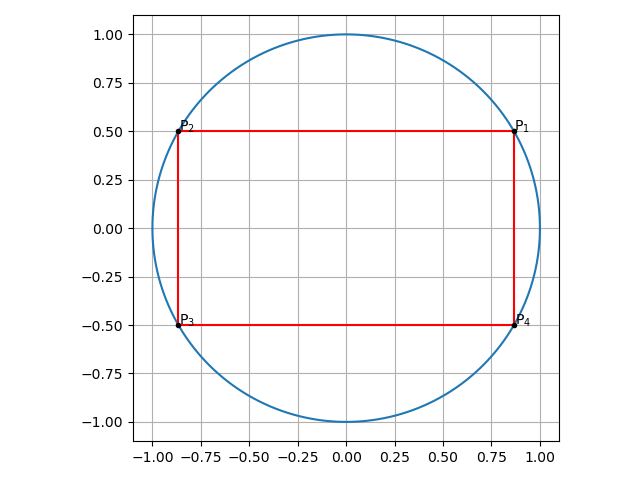
\includegraphics[width=\columnwidth]{chapters/9/10/5/12/figs/circle.png}
        \caption{$P_1P_2P_3P_4$ is a rectangle.}
        \label{fig:chapters/9/10/5/12/circle}
    \end{figure}


\end{enumerate}
